
\begin{tikzpicture}[shorten >=1pt,draw=black!50, x=1cm, y=1 cm,  node distance=0cm]
	\draw[draw=none, use as bounding box](-2,0) rectangle (8,6);
	\def\layersep{2cm}
	
    \tikzstyle{every pin edge}=[<-,shorten <=1pt,thick]
    \tikzstyle{neuron}=[circle,fill=black!25,minimum size=0.5cm ,inner sep=0pt, color=black, draw]
    \tikzstyle{input neuron}=[neuron, fill=green!50!blue!50];
    \tikzstyle{output neuron}=[neuron, fill=green!50!blue];
    \tikzstyle{hidden neuron}=[neuron, fill=green!50!orange];
    \tikzstyle{annot} = [text width=2em, text centered]
	\begin{scope}[x=1cm,y=1cm]
    % Draw the input layer nodes
    \foreach \name / \y in {2,3,4}
        \node[input neuron,fill=orange!100 ] (I-\name) at (0,\y) {$ $};

	 % Draw the hidden layer nodes
	 \foreach \name / \y in {1,2,3,4}
		 \path[yshift=0.5] node[hidden neuron] (H-\name) at (\layersep,\y+0.5) {\small $ $};
	 \foreach \name / \y in {1,2,3,4}
		 \path[yshift=0.5] node[hidden neuron] (H2-\name) at (2*\layersep,\y+0.5) {\small $ $};
	 \foreach \name / \y in {1,2,3,4}
		 \path[yshift=0.5] node[hidden neuron] (H3-\name) at (3*\layersep,\y+0.5) {\small $ $};
	 
	 % Draw the output layer node
	 \node[output neuron,pin={[pin edge={->}]right:\footnotesize Output}] at (4*\layersep,3) (O) {$ $};

	 \foreach \dest in {1,2,3,4}     
		 \foreach \source in {1,2,3,4}
		 {
			 \path[thick,->,gray] (H-\source) edge node[font=\scriptsize] {} (H2-\dest) ;
			 \path[thick,->,gray] (H2-\source) edge node[font=\scriptsize] {} (H3-\dest) ;
		}
 %        \foreach \dest in {2,4,6,8}

	 \end{scope}	             
    \foreach \source in {1,2,3,4}
           \path[thick,->,gray] (H3-\source) edge node[font=\scriptsize] {} (O) ;
    \foreach \source in {2,3,4}
		\foreach \dest in {1,2,3,4}     
        	\path[thick,->,gray] (I-\source) edge node[font=\scriptsize] {} (H-\dest) ;
%    % Annotate the layers
	\node [] (ll) at (-1.25,3) {RAC-155};
	\node[circle, black,thick,minimum width = 2.7cm,minimum height = 2.7cm,path picture={\node at (path picture bounding box.center){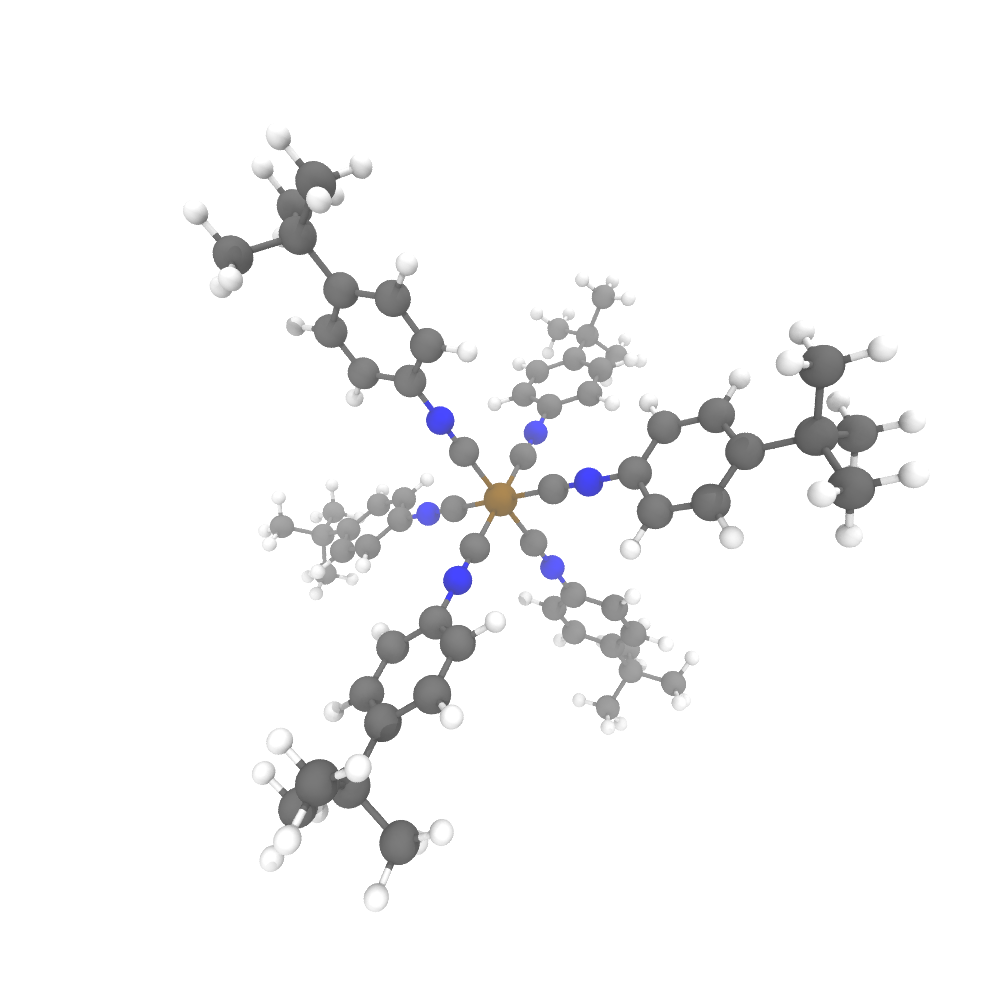
\includegraphics[width=3cm]{representations/images/pisc_trans}}; }] (Xp) at (-1.24,4) {};
% 	\node [] (ll) at (-1.25,1) {MOLECULE};
\end{tikzpicture}